\documentclass[11pt,onecolumn]{article}
\usepackage[english]{babel}
\usepackage[utf8]{inputenc}
\usepackage[T1]{fontenc}
\usepackage{amsmath,amssymb,amsfonts}
\usepackage{fullpage}
\usepackage{listings}

\usepackage{xspace}
\usepackage{graphicx}
\usepackage{color}
\usepackage{geometry}
\newcommand{\system}{MADden\xspace}

\newcommand{\ceg}[1]{{\textcolor{green}{#1 -- CEG}}}

\title{MADden : In-Database Text Analytics}
\author{Morgan Bauer 9890-4838 \\
  Christan Grant 8143-3970 \\
  Joir-dan Gumbs 6148-9357}
\date{December 13, 2011}
\begin{document}
\maketitle

\begin{figure}
  \begin{center}
    %
\includegraphics[width=104mm]{logo.jpg}
    
\includegraphics[width=40mm]{logo.jpg}
   %
\includegraphics[width=4cm]{logo.jpg}
    \caption{Logo for overarching project.}
    \label{fig:logo}
  \end{center}
\end{figure}


\begin{abstract}
In many domains, structured data and unstructured text are
both important natural resources to fuel data analysis. Statistical
text analysis needs to be performed over the text data to extract
structured information for further query processing. Common practice
in industry requires developers to connect multiple tools to build
off-line batch processes to perform such analysis tasks. \system is
an integrated system for ad hoc real-time query processing over
structured and unstructured data. \system is built on top of MADlib,
and PostgreSQL, and integrates in-database text extraction
techniques from BayesStore. 
We developed a web site that demonstrates queries using different
textual analytic tasks.
\end{abstract}


  \section{Introduction}

  \textbf{\system, MAD, Magnetic Agile Deep.}
  Mad Libs is a classic fill in the blank game that usually have amusing and unforeseen outcomes.
  In the \system project, our initial problem domain deals with football,
  and John Madden is a hall of fame coach, former player, and former commentator.
	He is most popular
  for the long-running series of video games that bear his name.

    There are large amounts of structured and unstructured data that is freely available,
		we create a proof of concept system to show how to intermix the two.
    We use statistical text analysis techniques to extract structured information from unstructured 
		data, and pass this on to later stages for further processing.

    We provide the ability to run queries over heterogeneous data such as structured statistical 
		fact tables and unstructured natural language. All the techniques are 
developed inside of the database and are executed using a SQL interface.
    Additionally, we  scrape dirty data and turn it into clean information, and then presenting 
		the information in an easy to digest form.
    We want to create queries over sports data to gain insight of a player and/or teams
		performance along with fan sentiment.
    We do however hope to be generic, and liberal in the data we take in, so that the same techniques can be applied to multiple domains.
    There is a web interface that provides pre-created web form queries that can be filled in 
		like the Mad Libs game \footnote{http://www.cise.ufl.edu/~cgrant/MADden}.
    It serves as a proving ground for various queries we test and run.
		Additionally, we create visualization of the results in html and using
interactive web charts.


Each author contributed to the building \system.
   \textbf{Morgan} did consulting work among the various group members, and between groups.
    Official NFL team blogs. NFL stats from cbssports.com. He also led in the creation of the paper.
		\textbf{Christan} built the \system website including the Mad lib style interface and the 
		result page with the charts and graphs. He obtained the tweet corpus, created the functionality
		for entity resolution, information extraction, and sentiment analysis. He also helped Morgan
		write the final paper.
		\textbf{Joir-dan} Joir-dan obtained play-by-play data from ESPN.com, CBS sports, blogs,
		and news recap articles.
		He also came up with queries for the web site.


  \section{Background}
  \subsection{Domain}

  Our initial domain is a sports domain and more specifically the National Football League (NFL).
  This domain is relevant for to sports journalist to do computational journalism.
  Covering all 32 teams with more than 1700 players is a time consuming task.
  A sports journalist would need a system
  that can analyze both the
  structured statistics (e.g., scores, biographic data) of teams and players and the
  unstructured tweets, blogs, and news about the games.
	Additionally, a coaches and scouts would find use in creating statistical queries over NFL data.



  \subsection{Background Information}

    Text analysis uses the state-of-the-art statistical machine learning (SML) methods to extract structured information,
    such as entities, relations, sentiments, topics, from text.

    The result of the text analysis can be joined with other
    structured data sources to perform analysis. For example, the sports
    journalist may want to join the sentiment result from tweets and the
    scores of the Arizona Cardinals\footnote{http://www.azcardinals.com}
    (NFL Team) to see their correlations.
		Below we discuss the algorithms we use.

  \begin{enumerate}

  \item Part of Speech (POS) Tagging

	We used part of speech taking from the natural language toolkit (NLTK). 
	The calls for POS tagging was wrapped into a Postgres user-defined function.


  \item Sentiment

    Sentiment analysis extracts the polarity of subjective opinions from documents.
    These subjective feelings are important for assessing the popularity of subjects,
    and can be used to establish the collective feelings of the public on a subject.


  \item Information Extraction (IE) 

	IE is the concept of identifying objects of interest,
    using relations present in the data.
    This varies from simple relations between subjects,
    to recognizing specific entities within text.
		For example, we may want to extract all the `organizations' mentioned in 
		a news article.


  \item Entity Resolution (ER) 
	
		ER is the processing of recognizing and disambiguating different subjects in a document.
    That is, recognizing that people are present,
    or mentioned, and knowing who they are.

    Where as IE was concerned about the existence of various objects,
    and identifying their existence,
    ER is concerned with taking these entities and knowing whether they are the same or different.
		In may situations, the output of information extraction becomes the input 
		to an entity resolution task.


  \item Conditional Random Fields (CRF) are a type of graphical model.
    A CRF is a supervised learning algorithm, requiring labeled training examples.
    In our case we are using CRFs to label sequences of natural language text.
    The quality and breadth of this set determines how well the trained CRF performs.
    They can be used for different things depending on their training set.
    We intended to use CRFs for POS tagging, IE, and ER.

     \end{enumerate}
  \subsection{Related work}

Several similar systems have been created by companies for 
internal and specific tasks
As far as we know, \system is the only system to integrate as much text analytic
tasks into a single query interface allowing the ability to 
create ad hoc queries, as if they fit.
  This is a ``what we want, not how to get it'' style query.

In computational journalism, the panda project\footnote{http://blog.apps.chicagotribune.com/}  
is a new effort to allows journalists to search and find relationship between 
many news stories. However, their system does not provide the same type of 
query interface.
The TweeQL project was created at MIT and it allowed a query interface for 
sentiment analysis over tweets\cite{Marcus:2011:TDD:1989323.1989470}. 
They developed an SQL like language for stream query preprocessing over the 
sampled the live twitter stream.

Daisy Wang \cite{wang2011hybrid} developed in-database techniques for 
conditional random fields. Our system aim to also have a completely in-database
text analytics stack.


  \section{System Description }
  \subsection{Architecture}

  {\system} is a four layered system, as can be seen in Figure \ref{fig:arch}.
  The user interface is where both naive and advanced users can construct queries over text, structured data, and models.
  From the user interface,
  queries are then passed to the DBMS,
  where MADLib \footnote{http://madlib.net/} and {\system} libraries sit on top of the query processor to add statistical and text processing functionality.
  % These queries are processed using PostgreSQL/Greenplum's Parallel DB architecture to further optimize on replicated storage.


  \subsection{System Components}
  %What are the system components and statistical methods developed?

  \system uses PostgreSQL, with MADlib overtop.
  We hope to scale up and use Greenplum massively parallel processing database.

  There is a new feature for MADlib that implements CRF evaluation, but not 
	training, in the database.
  The full text search capabilities of PostgreSQL are leveraged,
  as is the technique of inverted indexing.

	In addition, we developed our own text analytic functions, these are
	described below.

    \subsubsection{Information Extraction}

    Once we have the text documents, we would like to then be able to identify
    objects of interest. Information Extraction methods become increasingly
    important as the size of our corpus gets large. Many methods exist for in-database data
    extraction, but we are currently focused on building upon existing work in
    utilizing Conditional Random Fields (CRFs) for query-time extraction of
    entities.

    This is applied to the unstructured twitter data,
    and the semi-structured play-by-play data.
    As well, this would be applied for Named Entity Recognition purposes to general text, for identifying players and teams.
		Presently, we rely on models built by nltk to perform part-of-speech 
		tagging and subsequently information extraction. NLTK can label 
		terms and tag them with the label type. 


    \subsubsection{Entity Resolution}
    \label{sec:SCER}

    ER links various forms and representations of the same background object,
    so that a query for one of them returns the results for all of them.
    This is necessary for two reasons,
    the informality of speaking in documents like blog posts and twitter tweets,
    which leads to misspellings and slang
    and the more  general case of people or companies having many names to refer to them.

    An example of the informality of the slang and misspellings in twitter is
		``tmrw'' for ``tomorrow'' and ``NY Jest'' vs ``NY Jets''. Sometime 
		misspellings are intensional.

    An example of a person having multiple names is the
    nickname for Larry Fitzgerald which is ``Sticky Fingers''.
		Companies may also have acronym and nickname
    for example ``International Business Machines'' vs ``IBM'' vs ``Big Blue''
    and ``New York City'' vs ``Big Apple''.

    An example of multiple things with one name is
    Arizona Cardinals vs cardinals as a bird,
    Miami Dolphins vs dolphins as a fish and dolphins as a mammal.

    This is implemented through qgrams for misspellings and alternate spellings,
    and an alias table for multiple names of an entity.
    qgrams is the automatic approach that does fuzzy string matching,
    with a threshold value that can be varied.
    The alias table being hand constructed.


    \subsubsection{Q-grams}
    \label{qgram}

		Qgrams also known as character ngrams is implemented inside of the database.
		This technique as an approximate string match was first introduced in the 
		SQouT project \cite{Jain:2009:BQO:1519103.1519108}.
		To create qgrams over text in SQL we generate possible string and use the 
	substring utilities to trim the correct gram.
		We are implement it in purely in the database as a user defined function
		 so it works well with MPP systems.
		Given a string ``\textcolor{blue}{Tim Tebow}'' we can create a 3-gram by 
		using a sliding window. We show the out put in figure \ref{tab:qgramoutput}.
	
		\begin{figure}	
\begin{center}
		\begin{tabular}{|l|l|}
		\hline
		\textbf{Position} & \textbf{3-gram} \\
		\hline
		$1$ & \#\#T \\
		\hline
		$2$ & \#TI \\
		\hline
		$3$ & TIM \\
		\hline
		$4$ & IM\_ \\
		\hline
		$5$ & M\_T \\
		\hline
		$6$ & \_TE \\
		\hline
		$7$ & TEB \\
		\hline
		$8$ & EBO \\
		\hline
		$9$ & BOW \\
		\hline
		$10$ & OW\% \\
		\hline
		$11$ & W\%\% \\
		\hline
		\end{tabular}
\end{center}
\caption{Qgrams creation for the term 'Tim Tebow'}
\label{tab:qgramoutput}
		\end{figure}

Given two tables we can compare the overlap of two qgrams and compute a
similarity. The we compute the similarity between $term_1$ and $term_2$
using the equation
$$ S(term_1,term_2) = 
\frac{|term_1 \cap term_2|}{\min\{|term_1|, |term_2|\}} .$$

Qgram approach may fail with small words with error in the center. An 
example of this is displayed in the VOTKA vs VODKA figure \ref{tab:vodka}.

	\begin{figure}
\begin{center}
    \begin{tabular}{|c|c|}
		\hline
      \textbf{VOTKA} & \textbf{VODKA} \\ \hline
      {\color{blue}\#\#V} & {\color{blue}\#\#V} \\
		\hline
      {\color{blue}\#VO} & {\color{blue}\#VO} \\
		\hline
      {\color{red}VOT} &  {\color{red}VOD} \\
		\hline
      {\color{red} OTK} &{\color{red} ODK} \\
		\hline
      {\color{red} TKA} &{\color{red} DKA} \\
		\hline
      {\color{blue}KA\$} & {\color{blue}KA\$} \\
		\hline
      {\color{blue}A\%\%} &  {\color{blue}A\%\%} \\
		\hline
    \end{tabular}
\end{center}
\caption{An example of an unfortunate error situation in qgrams} 
\label{tab:vodka}
	\end{figure}

In general the qgram approach is very approximate and loses accuracy with
large documents.
Run time for search is $O(|T|*|P|)$ where $|T|$ and $|P|$ is the text and
search pattern. We believe that creating indices over the document qgrams
will help the run-time. 
For large documents we can do hashing tricks to avoid super large 
joins between data sets.  


    \subsubsection{Sentiment Analysis}
    \label{sec:SCSA}

    Sentiment analysis extracts the polarity of subjective opinions from documents.
    The current implementation returns sentiment as a trinary option of positive, neutral, or negative.
    We would like to have more gradations in the extremeness of the opinion,
    as well as analysis of an opinion pertaining to a certain subject, or entity, that has been extracted.

    Currently, this is handled as a UDF which makes an out of database call across the network.
    It also does this on a document by document basis,
    when the submission API supports batches of documents\footnote{https://sites.google.com/site/twittersentimenthelp/}.
    Priority should be given to establish batch submissions,
    followed by writing the UDF as a local function,
    and possibly an in-database function.

    \subsubsection{Part of Speech Tagging}
    Part of Speech Tagging (POS tagging) labels each token of a sequence with a tag based on the grammar of a natural language.
    These tags are parts of speech, based on context and word definitions.
    The generators for these tags can come from both supervised and unsupervised sources.
    Statistical methods are used to generate taggers specific to a corpus, and thus a particular subject.
    These parts of speech are useful in other stages, such as entity resolution and information extraction (ER \& IR).

    
    The model was initially trained on email headers.
    This data was not generic enough to be useful in our tweet and news corpus.
    The individual documents were to small and not of a form similar enough to ensure correct tags.

    The next CRF was trained using email contents.
    While it had a higher accuracy, the training corpus was still too
		small at only 100 or 200 documents.

    We need to train a CRF specific to our domain,
    and would like to train a CRF specific to each type of text,
    such as a twitter CRF, a blog CRF, etc.

  \begin{figure}
    \begin{center}
      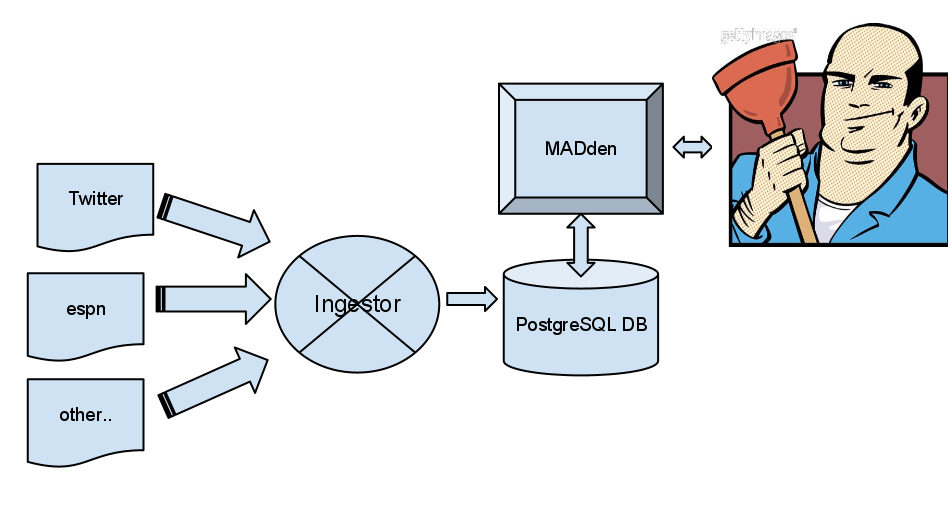
\includegraphics[width=104mm]{architecture-1.png}
      \caption{Original System Architecture}
      \label{fig:architecture}
    \end{center}
  \end{figure}

  \begin{figure}
    \begin{center}
      \includegraphics[scale=0.4]{arch.png}
      \caption{{Our updated \system} architecture}
      \label{fig:arch}
    \end{center}
  \end{figure}


  \begin{figure}
    \begin{center}
      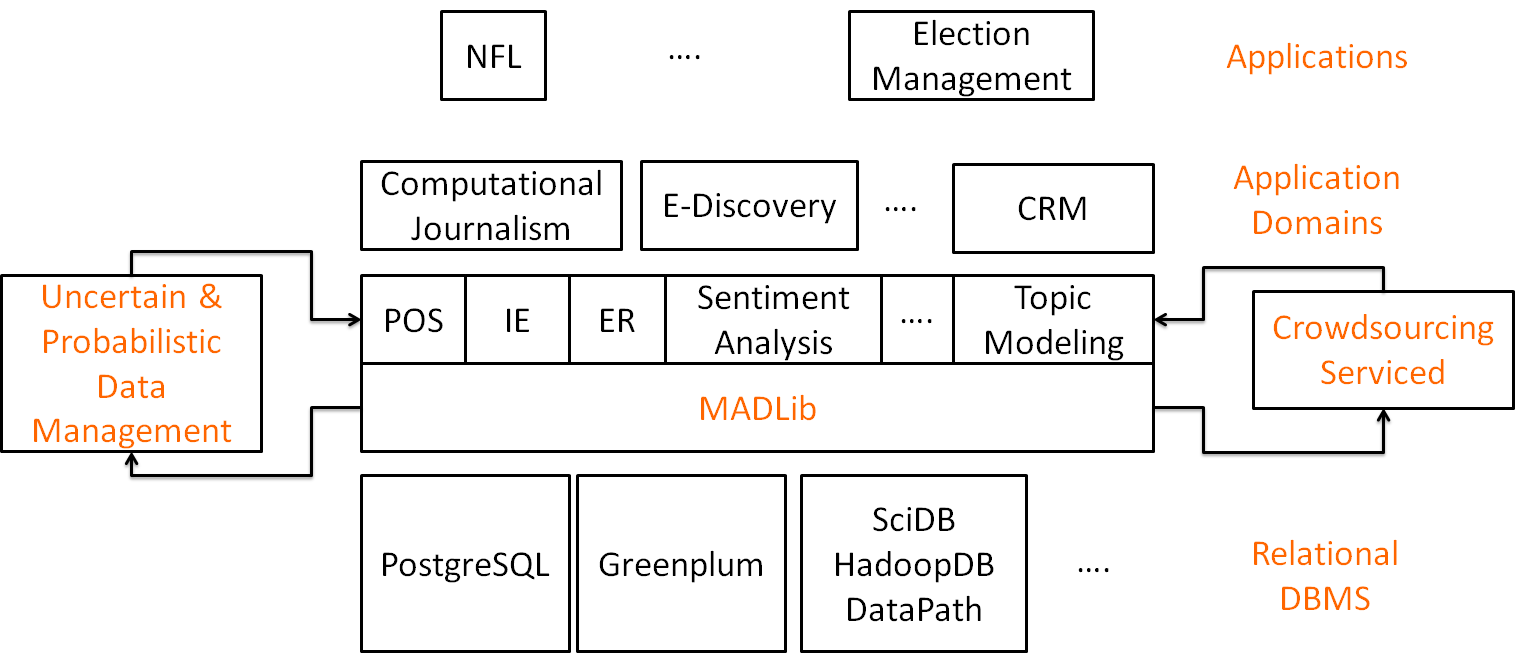
\includegraphics[scale=0.3]{altachitecture.png}
      \caption{Overall {\system} architecture}
      \label{fig:altarch}
    \end{center}
  \end{figure}


  %\begin{figure}
  %  \begin{center}
  %    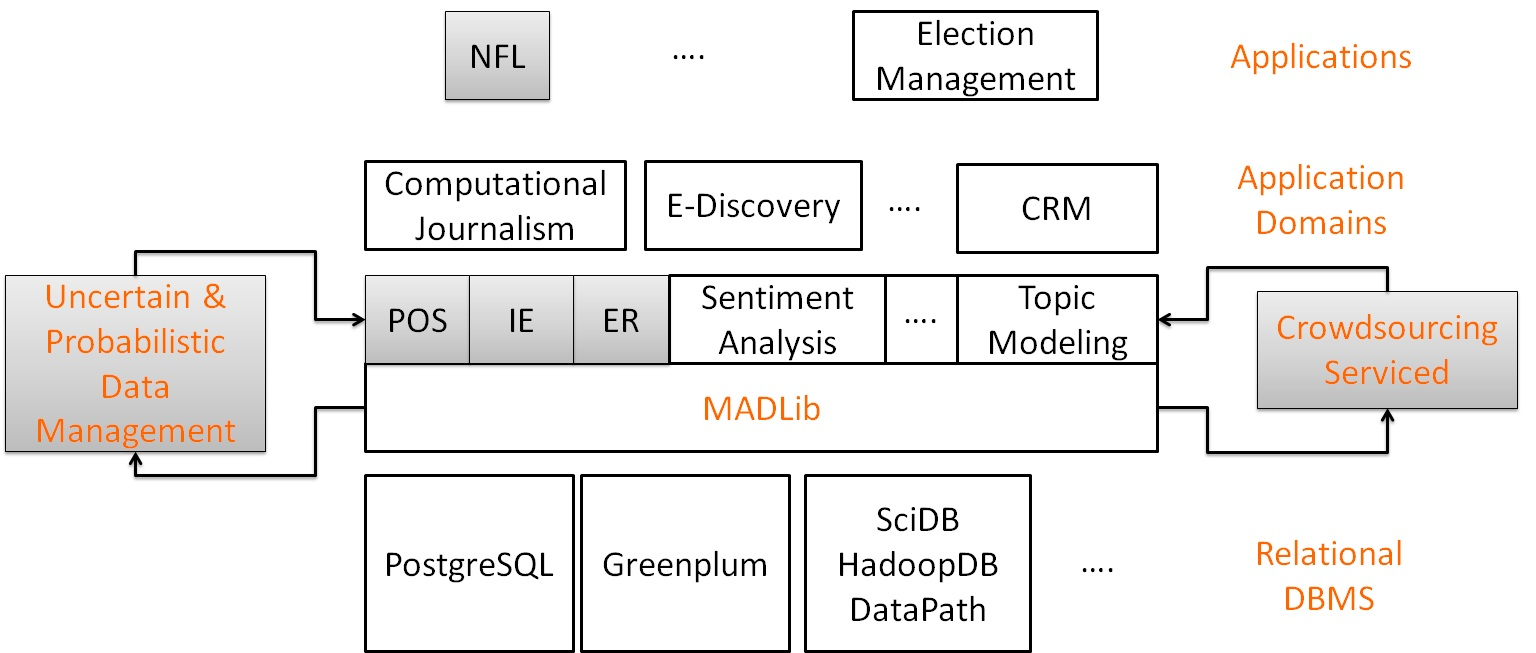
\includegraphics[scale=0.3]{altarchitecture2.jpg}
  %    \caption{{\system} architecture 2}
  %    \label{fig:altarch2}
  %  \end{center}
  %\end{figure}



  \subsection{Data Products}

	We created a set of tools to query over data and extract knowledge.
	We created a website to interface with the database and visualize results.

	We developed 5  Mad Lib style queries including;
	\begin{enumerate}
	\item Give me [number] [+/-/o] sentiment comments about [Player].
	\item Compare [Player1][Player2] by the twitter sentiment	over dates from
	[from] and [to] and return [number] results.
	\item Give me the [+/-/o] sentiment for the top [number] 
	[running back/quarter back/ wide receiver] for tweets.
	\item Return all the named entity tags from the text [text].
	\item Give me th [number] tweets and their sentiment corresponding to 
	one of the top [number]  [running back/quarter back/ wide receiver].
	\end{enumerate}

	Each of these queries map directly to SQL queries that we run on our system.
The queries are:
	\begin{enumerate}
	\item 
{\small
\begin{verbatim}
SELECT cgrant_sentiment(twtext) as sent, twtext, twuser_id_str, id_str
FROM tweets
WHERE (cgrant_distance(1,[player],2, twtext, 5) > .5)
AND cgrant_sentiment(twtext) = [+/-/o]
GROUP BY sent, text
LIMIT [number];	
\end{verbatim}
}
	\item
{\small
\begin{verbatim}
SELECT (CASE WHEN 
(cgrant_distance(1,[Player1],2, twtext, 5) > .5) THEN '[Player1]'
ELSE '[Player2]' END), created_at, cgrant_sentiment(twtext), twtext
FROM tweets
WHERE created_at between [from] and [to]
AND ((cgrant_distance(1,[Player1],2, twtext, 5) > .5) OR ".
(cgrant_distance(1,[Player2],2, twtext, 5) > .5)) LIMIT [num];
\end{verbatim}
}

	\item
{\small
\begin{verbatim}
SELECT id, fname, lname, yards, tds, doc, sentiment FROM
(SELECT id, fname, lname, yards, tds, doc, cgrant_sentiment(doc) AS sentiment
FROM
(SELECT rb.pid as id, rb.first as fname, rb.last as lname, n.twtext as doc, 
rb.total_yards as yards, rb.touchdowns as tds 
FROM tweets n, 
(SELECT pid, first, last, total_yards, touchdowns, first || ' ' || last as tsv
FROM [running back/quarter back/wide receiver table] 
ORDER BY total_yards DESC, touchdowns DESC
LIMIT [number]) as rb 
WHERE cgrant_distance(1, rb.tsv, 2, n.twtext, 5) > .5) as docs) as sent 
WHERE sentiment = [+/-/o]
LIMIT [number];

\end{verbatim}
}
	\item
{\small
\begin{verbatim}
SELECT termnum, term
FROM cgrant_ne_chunk('[comments]', true)
WHERE tag = 'NE' ;
\end{verbatim}
}
	\item
{\small
\begin{verbatim}
SELECT topKplayers.full_name, twtext, cgrant_sentiment(twtext) 
FROM tweets, (SELECT first || ' ' || last as full_name, total_yards, touchdowns
FROM [running back/quarter back/wide receiver table] 
ORDER BY total_yards DESC, touchdowns DESC 
LIMIT [K]) as topKplayers 
WHERE cgrant_distance(1, topKplayers.full_name, 2, twtext, 5) > .5 
LIMIT [number];
\end{verbatim}
}
	\end{enumerate}

	
	In addition, we have seven queries that are made possible in the \system system. They are listed in the appendix section \ref{sec:extraqueries}.

  \begin{figure}
    \begin{center}
      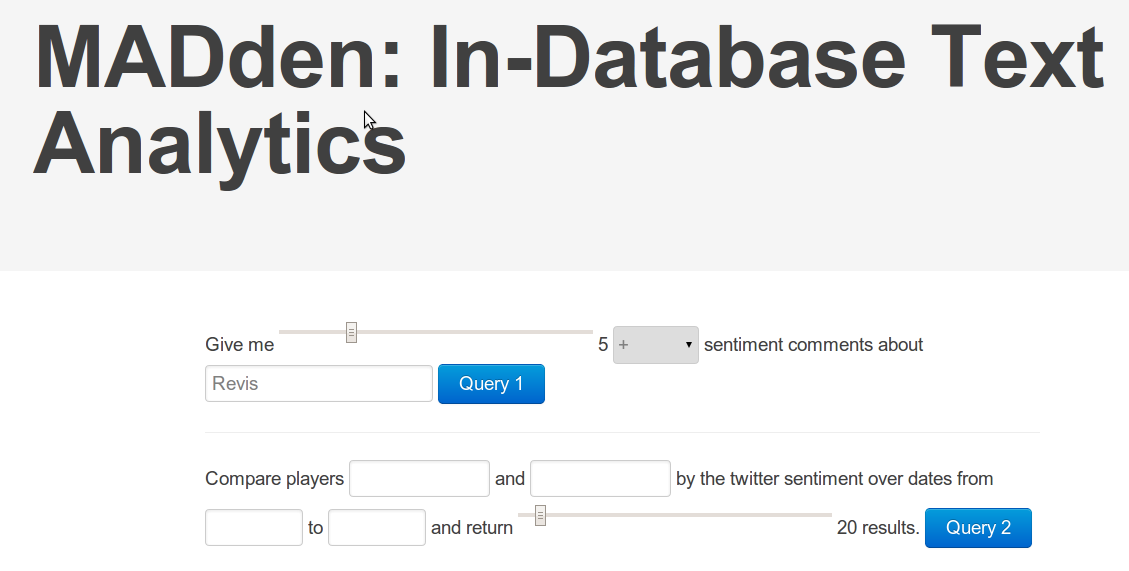
\includegraphics[scale=0.3]{web-ui.png}
      \caption{{\system} Web UI}
      \label{fig:web-ui}
    \end{center}
  \end{figure}

  \section{Experiments}

		We obtained data from several different data sources.
		We obtained over 20,916,048 tweets from the Twitter API.
Each tweet has a maximum of 140 characters as well as other metadata.
We obtained the data by searching football related terms on the tweet stream.
The tweets were collected during NFL game days from August 18th to
November 29th. The data amounted to 
approximately 9GB of tweets, yielding a 7GB inverted index.

We obtained blogs from 20 of the 32 teams. The blogs were all english
language and documents are each between 10-100 sentences.
There are over 33 thosand unique articles at 186 MB. 
We also have information from ESPN, CBSSports, and NFL.com. This data includes
60,680 news and opinion articles and play-by-play information from 530 games.
The play-by-play data has repeated patterns with specific meaning.

    Throughput for sentiment analysis is dominated by making a remote call.
    Throughput for POS tagging is dominated by making a python call and 
loading the NLTK into memory (interpreted).
The queries involving tweets take along time to complete because of the shear
size of the tweet tables.


  \section{Conclusion}
We developed \system, a system that allowed anyone do perform advanced
queries over structured and unstructured text.
We included data over several different types in the NFL domain.

    Each member of the team had a unique experience taking the large scale
data science class and developing \system.
		Morgan learned how to parse html, write and use a web crawler, 
		He learned about conditional random fields stuff and how to setup and use
		the Postgresql DBMS. He also experienced that it is a difficult task to
		obtain and clean data.
		Christan learned how to create complicated sql queries. 
He also learned to develop AJAX calls for dynamic Web 2.0 style 
web site creation.
Additionally, he learned how to wrap almost 
		anything in a posgres UDF. 
		Joir-dan learned that Databases are fickle, text analytics are pretty sweet and have a great upside.

As future work we will run the queries on a massively parallel processing 
database offered by Greenplum\footnote{http://www.greenplum.com}.
In addition we plan to expand the website
to allow users to create account and develop their own Mad Lib style 
queries as well as visualizations.
The information extraction and sentiment analysis is not yet in the database
we plan to develop in database techniques to facilitate scale.

\bibliographystyle{abbrv}
\bibliography{citation.bib}

\appendix

\section{Extra Queries}
\label{sec:extraqueries}
Here is a list of extra queries and an explanation developed for \system.
The first query is an example of a search using an inverted index.
\begin{verbatim}
-- We want to find 10 queries that contain the Running Back 
-- 'Maurice Jones-Drew' (exact match only)
SELECT twtext FROM tweets
WHERE twtextvector @@ to_tsquery('Maurice & Jones-Drew')
LIMIT 10;
\end{verbatim}


This query is an example of entity resolution using qgrams and approximate 
string matching. This shows up inside of the ``cgrant\_distance'' function.
\begin{verbatim}
-- We want to find 10 queries that contain the Running Back 
-- 'Maurice Jones-Drew' (allow distance of at least .5 (resoluting) )
SELECT twtext 
FROM tweets
WHERE cgrant_distance(1, 'Maurice Jones-Drew', 2, twtext, 4) > .5
LIMIT 10;
\end{verbatim}


This query is an example of using the sentiment analysis function.
\begin{verbatim}
-- Give me the sentiment for the first 100 tweets we have
SELECT cgrant_sentiment(twtext)
FROM tweets
LIMIT 100;
\end{verbatim}


This query uses both entity resolution in a more complicated query.
\begin{verbatim}
-- Give me the first 100 tweets containing one of the top ten 
-- Quarterbacks in passing yards (we need to extract names, and then 
-- resolute the names in the tweet)
SELECT topKplayers.full_name, twtext FROM tweets, 
	(SELECT first || ` ' || last as full_name, total_yards, touchdowns
              FROM passingstats
              ORDER BY total_yards DESC, touchdowns DESC
              LIMIT 10) as topKplayers
WHERE cgrant_distance(1, topKplayers.full_name, 2, twtext, 5) > .5
LIMIT 100;
\end{verbatim}


This query mixes information extraction, using the inverted index as well
as sentiment analysis through the user defined function.
\begin{verbatim}
-- Give me the first 20 tweets containing the Quarterback 'David Garrard' 
-- that is not a retweet, and give me the sentiment for each tweet
SELECT twtext, cgrant_sentiment(twtext)
FROM tweets
WHERE twtextvector @@ to_tsquery(`David & Garrard & !RT')
LIMIT 20;
\end{verbatim}

This query uses both information extraction and entity resolution.
\begin{verbatim}
-- Give me the tweets and sentiment of the first 20 tweets that contain the 
-- Quarterback `Tim Tebow'  (resoluted name)
SELECT twtext, cgrant_sentiment(twtext)
FROM tweets
WHERE cgrant_distance(1, `Tim Tebow', 2, twtext, 5) > .6
LIMIT 20;
\end{verbatim}

This query uses information extraction, entity resolution
and sentiment analysis.
\begin{verbatim}
-- Information Extraction with Entity Resolution with Sentiment Analysis
-- Give me the tweets and sentiment for the first 20 tweets that contain 
-- the Quarterback `Tim Tebow' (Resoluted) and contains the `#Jaguars' hashtag
SELECT twtext, cgrant_sentiment(twtext)
FROM tweets
WHERE cgrant_distance(1, `Tim Tebow', 2, twtext, 5) > .6 
AND twtextvector @@ to_tsquery(`#Jaguars')
LIMIT 20;
\end{verbatim}



\end{document}

